\chapter{Deep learning glossary}
\label{app:dl_glossary}

\graphicspath{{images/appendix/}, {tikz/appendix/} }

\subsubsection*{Attention} \label{gl:attention}

Attention \citep{Vaswani2017} is, informally, a technique that allows a neural network to "focus" on a subset on the inputs by masking parts of the input vector. The most common type of attention is computed using a dot product: let $\vx \in \spaceR^n$ be the input of a neural network layer $l(.)$. Dot product attention consists in weighting the output and $l(\vx) \in \spaceR^m$ of the layer $l$ with a feature vector $f_\theta(\vx) \in [0,1]^m$, where $f_\theta$ is typically a neural network, as

\begin{equation}
	l'(\vx) = l(\vx) \odot f_\theta(\vx) \enspace.
\end{equation}

\subsubsection*{Auto-encoder} \label{gl:ae}

Auto-encoders $AE(.)$ are a family of neural network architectures that are trained to copy its input to its output, as $AE(\vx) = \vx$. Since this is normally a trivial task, auto-encoders are constrained by their architecture (usually an \gl{encdec}{encoder-decoder} architecture with a low-dimension latent representation) or through regularization. The aim of auto-encoders is usually to learn a good representation model of the data.

\subsubsection*{Batch Normalization} \label{gl:batchnorm}

Batch Normalization \citep{Ioffe2015} is a normalization technique that consists in re-centering and re-scaling the input $\vx$ of a neural network layer. To approximate the mean and covariance of the full dataset, Batch Normalization computes ${\mu}_{mb}$ the mean and ${\sigma}_{mb}$ the variance of the data in present in the mini-batch. It also keeps two parameters, $\beta$ and $\gamma$, updated during the training of the neural network, and uses them to shift and scale the input as

\begin{equation}
	BN(\vx|\beta,\gamma) = \gamma\frac{\vx - {\mu}_{mb}}{\sqrt{{\sigma}_{mb}}} + \beta \enspace .
\end{equation}

\subsubsection*{Deconvolutional layer / Transposed convolution} \label{gl:deconv}

Deconvolutions \citep{Long2015}, or transposed convolutions, are the inverse operation of convolutions. As opposed to convolutions in which striding decreases the dimension of the feature maps, deconvolutions allows for filters to upscale the feature maps using striding.

\subsubsection*{Dilated convolution} \label{gl:dilconv}

\begin{figure}
	\centering
	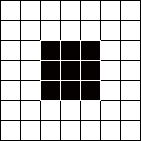
\includegraphics[width=\textwidth/5]{dilation1}\hspace{1cm}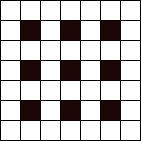
\includegraphics[width=\textwidth/5]{dilation2}\hspace{1cm}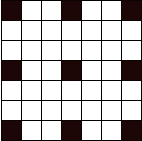
\includegraphics[width=\textwidth/5]{dilation3}
	\caption{ Dilated filters with dilation rate of 1, 2, 3}
	\label{fig:dilation}
\end{figure}

Dilated convolutions \citep{Yu2015} (or ``A trous'' convolutions) are convolutions in which the size of the filters receptive fields is artificially increased, without increasing the number of parameters, by using sparse filters (see Figure \ref{fig:dilation}). 

\subsubsection*{Encoder-decoder architecture} \label{gl:encdec} 

An encoder-decoder architecture is a neural network that consists in two parts: the encoder which downscales the input to a small dimension representation; and a decoder which upscales this small dimension representation to obtain a high-dimension output.

\subsubsection*{Instance Normalization} \label{gl:instnorm}

Instance Normalization \citep{Ulyanov2016} is a variant of Batch Normalization which does not compute the means and variances on the full mini-batch, but instead standardizes the input using the means and variances for a single input, across all dimensions.

\subsubsection*{Residual block} \label{gl:resblock}

\begin{figure}
	\centering
	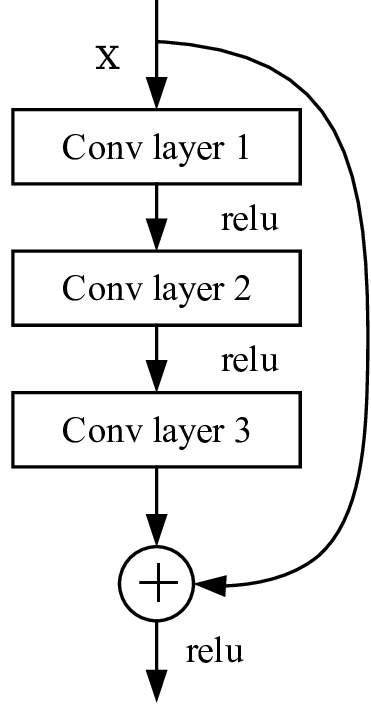
\includegraphics[height=6cm]{resnet}
	\caption{3 layer residual block}
	\label{fig:resblock}
\end{figure}

A residual block is a set of several layers with a skip-connection that links the first layer of the block to the last one (see Figure \ref{fig:resblock}). Residual blocks allow for having very deep neural network architectures while mitigating vanishing gradient issues.

\subsubsection*{Skip connection} \label{gl:skip}

Used in \glnf{ae}{auto-encoder} architectures and \glnf{resblock}{residual blocks}, a skip-connection allow for connecting the input of a layer $L_n$ to the input of another layer $L_m$ further up the network (see Figure \ref{fig:resblock}). This bypassed information can be aggregated to the input of $L_m$ using addition or concatenation. Skip-connections are used to allow for information to flow more easily up the network and is a way to mitigate vanishing gradient problems.

\subsubsection*{UNet} \label{gl:unet} A UNet  \citep{Ronneberger2015} is an \gl{encdec}{Encoder-Decoder} architecture with \glnf{skip}{skip-connections} between layers of the encoder and the decoder.